% Options for packages loaded elsewhere
\PassOptionsToPackage{unicode}{hyperref}
\PassOptionsToPackage{hyphens}{url}
%
\documentclass[
  stu]{apa7}
\usepackage{amsmath,amssymb}
\usepackage{iftex}
\ifPDFTeX
  \usepackage[T1]{fontenc}
  \usepackage[utf8]{inputenc}
  \usepackage{textcomp} % provide euro and other symbols
\else % if luatex or xetex
  \usepackage{unicode-math} % this also loads fontspec
  \defaultfontfeatures{Scale=MatchLowercase}
  \defaultfontfeatures[\rmfamily]{Ligatures=TeX,Scale=1}
\fi
\usepackage{lmodern}
\ifPDFTeX\else
  % xetex/luatex font selection
\fi
% Use upquote if available, for straight quotes in verbatim environments
\IfFileExists{upquote.sty}{\usepackage{upquote}}{}
\IfFileExists{microtype.sty}{% use microtype if available
  \usepackage[]{microtype}
  \UseMicrotypeSet[protrusion]{basicmath} % disable protrusion for tt fonts
}{}
\makeatletter
\@ifundefined{KOMAClassName}{% if non-KOMA class
  \IfFileExists{parskip.sty}{%
    \usepackage{parskip}
  }{% else
    \setlength{\parindent}{0pt}
    \setlength{\parskip}{6pt plus 2pt minus 1pt}}
}{% if KOMA class
  \KOMAoptions{parskip=half}}
\makeatother
\usepackage{xcolor}
\usepackage{graphicx}
\makeatletter
\def\maxwidth{\ifdim\Gin@nat@width>\linewidth\linewidth\else\Gin@nat@width\fi}
\def\maxheight{\ifdim\Gin@nat@height>\textheight\textheight\else\Gin@nat@height\fi}
\makeatother
% Scale images if necessary, so that they will not overflow the page
% margins by default, and it is still possible to overwrite the defaults
% using explicit options in \includegraphics[width, height, ...]{}
\setkeys{Gin}{width=\maxwidth,height=\maxheight,keepaspectratio}
% Set default figure placement to htbp
\makeatletter
\def\fps@figure{htbp}
\makeatother
\setlength{\emergencystretch}{3em} % prevent overfull lines
\providecommand{\tightlist}{%
  \setlength{\itemsep}{0pt}\setlength{\parskip}{0pt}}
\setcounter{secnumdepth}{-\maxdimen} % remove section numbering
% Make \paragraph and \subparagraph free-standing
\ifx\paragraph\undefined\else
  \let\oldparagraph\paragraph
  \renewcommand{\paragraph}[1]{\oldparagraph{#1}\mbox{}}
\fi
\ifx\subparagraph\undefined\else
  \let\oldsubparagraph\subparagraph
  \renewcommand{\subparagraph}[1]{\oldsubparagraph{#1}\mbox{}}
\fi
% definitions for citeproc citations
\NewDocumentCommand\citeproctext{}{}
\NewDocumentCommand\citeproc{mm}{%
  \begingroup\def\citeproctext{#2}\cite{#1}\endgroup}
\makeatletter
 % allow citations to break across lines
 \let\@cite@ofmt\@firstofone
 % avoid brackets around text for \cite:
 \def\@biblabel#1{}
 \def\@cite#1#2{{#1\if@tempswa , #2\fi}}
\makeatother
\newlength{\cslhangindent}
\setlength{\cslhangindent}{1.5em}
\newlength{\csllabelwidth}
\setlength{\csllabelwidth}{3em}
\newenvironment{CSLReferences}[2] % #1 hanging-indent, #2 entry-spacing
 {\begin{list}{}{%
  \setlength{\itemindent}{0pt}
  \setlength{\leftmargin}{0pt}
  \setlength{\parsep}{0pt}
  % turn on hanging indent if param 1 is 1
  \ifodd #1
   \setlength{\leftmargin}{\cslhangindent}
   \setlength{\itemindent}{-1\cslhangindent}
  \fi
  % set entry spacing
  \setlength{\itemsep}{#2\baselineskip}}}
 {\end{list}}
\usepackage{calc}
\newcommand{\CSLBlock}[1]{\hfill\break\parbox[t]{\linewidth}{\strut\ignorespaces#1\strut}}
\newcommand{\CSLLeftMargin}[1]{\parbox[t]{\csllabelwidth}{\strut#1\strut}}
\newcommand{\CSLRightInline}[1]{\parbox[t]{\linewidth - \csllabelwidth}{\strut#1\strut}}
\newcommand{\CSLIndent}[1]{\hspace{\cslhangindent}#1}
\ifLuaTeX
\usepackage[bidi=basic]{babel}
\else
\usepackage[bidi=default]{babel}
\fi
\babelprovide[main,import]{british}
% get rid of language-specific shorthands (see #6817):
\let\LanguageShortHands\languageshorthands
\def\languageshorthands#1{}
% Manuscript styling
\usepackage{upgreek}
\captionsetup{font=singlespacing,justification=justified}

% Table formatting
\usepackage{longtable}
\usepackage{lscape}
% \usepackage[counterclockwise]{rotating}   % Landscape page setup for large tables
\usepackage{multirow}		% Table styling
\usepackage{tabularx}		% Control Column width
\usepackage[flushleft]{threeparttable}	% Allows for three part tables with a specified notes section
\usepackage{threeparttablex}            % Lets threeparttable work with longtable

% Create new environments so endfloat can handle them
% \newenvironment{ltable}
%   {\begin{landscape}\centering\begin{threeparttable}}
%   {\end{threeparttable}\end{landscape}}
\newenvironment{lltable}{\begin{landscape}\centering\begin{ThreePartTable}}{\end{ThreePartTable}\end{landscape}}

% Enables adjusting longtable caption width to table width
% Solution found at http://golatex.de/longtable-mit-caption-so-breit-wie-die-tabelle-t15767.html
\makeatletter
\newcommand\LastLTentrywidth{1em}
\newlength\longtablewidth
\setlength{\longtablewidth}{1in}
\newcommand{\getlongtablewidth}{\begingroup \ifcsname LT@\roman{LT@tables}\endcsname \global\longtablewidth=0pt \renewcommand{\LT@entry}[2]{\global\advance\longtablewidth by ##2\relax\gdef\LastLTentrywidth{##2}}\@nameuse{LT@\roman{LT@tables}} \fi \endgroup}

% \setlength{\parindent}{0.5in}
% \setlength{\parskip}{0pt plus 0pt minus 0pt}

% Overwrite redefinition of paragraph and subparagraph by the default LaTeX template
% See https://github.com/crsh/papaja/issues/292
\makeatletter
\renewcommand{\paragraph}{\@startsection{paragraph}{4}{\parindent}%
  {0\baselineskip \@plus 0.2ex \@minus 0.2ex}%
  {-1em}%
  {\normalfont\normalsize\bfseries\itshape\typesectitle}}

\renewcommand{\subparagraph}[1]{\@startsection{subparagraph}{5}{1em}%
  {0\baselineskip \@plus 0.2ex \@minus 0.2ex}%
  {-\z@\relax}%
  {\normalfont\normalsize\itshape\hspace{\parindent}{#1}\textit{\addperi}}{\relax}}
\makeatother

\makeatletter
\usepackage{etoolbox}
\patchcmd{\maketitle}
  {\section{\normalfont\normalsize\abstractname}}
  {\section*{\normalfont\normalsize\abstractname}}
  {}{\typeout{Failed to patch abstract.}}
\patchcmd{\maketitle}
  {\section{\protect\normalfont{\@title}}}
  {\section*{\protect\normalfont{\@title}}}
  {}{\typeout{Failed to patch title.}}
\makeatother

\usepackage{xpatch}
\makeatletter
\xapptocmd\appendix
  {\xapptocmd\section
    {\addcontentsline{toc}{section}{\appendixname\ifoneappendix\else~\theappendix\fi\\: #1}}
    {}{\InnerPatchFailed}%
  }
{}{\PatchFailed}
\keywords{keywords\newline\indent Word count: X}
\usepackage{csquotes}
\usepackage[titles]{tocloft}
\cftpagenumbersoff{figure}
\renewcommand{\cftfigpresnum}{\itshape\figurename\enspace}
\renewcommand{\cftfigaftersnum}{.\space}
\setlength{\cftfigindent}{0pt}
\setlength{\cftafterloftitleskip}{0pt}
\settowidth{\cftfignumwidth}{Figure 10.\qquad}
\cftpagenumbersoff{table}
\renewcommand{\cfttabpresnum}{\itshape\tablename\enspace}
\renewcommand{\cfttabaftersnum}{.\space}
\setlength{\cfttabindent}{0pt}
\setlength{\cftafterloftitleskip}{0pt}
\settowidth{\cfttabnumwidth}{Table 10.\qquad}
\makeatletter
\renewcommand{\paragraph}{\@startsection{paragraph}{4}{\parindent}%
  {0\baselineskip \@plus 0.2ex \@minus 0.2ex}%
  {-1em}%
  {\normalfont\normalsize\bfseries\typesectitle}}

\renewcommand{\subparagraph}[1]{\@startsection{subparagraph}{5}{1em}%
  {0\baselineskip \@plus 0.2ex \@minus 0.2ex}%
  {-\z@\relax}%
  {\normalfont\normalsize\bfseries\itshape\hspace{\parindent}{#1}\textit{\addperi}}{\relax}}
\makeatother
\setlength{\cslhangindent}{0.5in}
\usepackage{fancyhdr} 
\pagestyle{fancy}   
\fancyhf{} 
\fancyhead[R]{\thepage} 
\renewcommand{\headrulewidth}{0pt}
\thispagestyle{fancy}
\duedate{07.08.2023}
\course{Modul 6b: Empirisch-Experimentelles Praktikum}
\professor{Dr. Sarina Schäfer}

\ifLuaTeX
  \usepackage{selnolig}  % disable illegal ligatures
\fi
\usepackage{bookmark}
\IfFileExists{xurl.sty}{\usepackage{xurl}}{} % add URL line breaks if available
\urlstyle{same}
\hypersetup{
  pdftitle={The title},
  pdfauthor={First Author1 \& Ernst-August Doelle1,2},
  pdflang={en-GB},
  pdfkeywords={keywords},
  hidelinks,
  pdfcreator={LaTeX via pandoc}}

\title{The title}
\author{First Author\textsuperscript{1} \& Ernst-August Doelle\textsuperscript{1,2}}
\date{}


\shorttitle{Title}

\authornote{

Add complete departmental affiliations for each author here. Each new line herein must be indented, like this line.

Enter author note here.

The authors made the following contributions. First Author: Conceptualization, Writing - Original Draft Preparation, Writing - Review \& Editing; Ernst-August Doelle: Writing - Review \& Editing, Supervision.

Correspondence concerning this article should be addressed to First Author, Postal address. E-mail: \href{mailto:my@email.com}{\nolinkurl{my@email.com}}

}

\affiliation{\vspace{0.5cm}\textsuperscript{1} Wilhelm-Wundt-University\\\textsuperscript{2} Konstanz Business School}

\note{\clearpage}

\abstract{%
One or two sentences providing a \textbf{basic introduction} to the field, comprehensible to a scientist in any discipline.
Two to three sentences of \textbf{more detailed background}, comprehensible to scientists in related disciplines.
One sentence clearly stating the \textbf{general problem} being addressed by this particular study.
One sentence summarizing the main result (with the words ``\textbf{here we show}'' or their equivalent).
Two or three sentences explaining what the \textbf{main result} reveals in direct comparison to what was thought to be the case previously, or how the main result adds to previous knowledge.
One or two sentences to put the results into a more \textbf{general context}.
Two or three sentences to provide a \textbf{broader perspective}, readily comprehensible to a scientist in any discipline.
}



\begin{document}
\maketitle

\section{Methods}\label{methods}

\subsection{Preregistration and version control}\label{preregistration-and-version-control}

The hypotheses, the inclusion/exclusion criteria, used databases, search queries and the basic theoretical foundation of this systematic literature review are preregistered and can be found on Moodle or in the GitHub repository.\\
As suggested by Lakens (2022) (Chapter 14), the present systemic literature used a GitHub repository to store all data and files. The repository is available at: \url{https://github.com/julianrottenberg/Stereotype_Threat_im_akademischen_Kontext}\\
This approach allows for more transparency and reproducibility as well as accountability.

\subsection{Artificial Intelligence (AI)}\label{artificial-intelligence-ai}

It should be acknowledged that artificial intelligence has been used as an aid in this review - namely, Anthropic's Claude AI 3.5 Sonnet (Anthropic, 2024) and GitHub's Copilot (GitHub \& OpenAi, 2024), the latter was directly integrated into RStudio Server (Posit team, 2024). The chats that directly influenced this review are all available on the GitHub repository.
For Github Copilot the autocomplete-style suggestions were used.\\
Claude AI 3.5 Sonnet was used to generate descriptions of the papers used in this review - based on a template.
The process here was as follows: First the template was manually filled out by a human, after this process was completed for every paper, a second template was created, the contents of which were filled out by AI and then, later, used in conjunction with the manually created templates. When the different templates differed from one another the primary source (i.e.~the paper the template was based on) was checked again. Both, the human-generated as well as the AI-generated templates can be found on the GitHub repository - the AI generated summaries have been marked as such, beginning with ``Claude\_Ai\_'' in their file name.\\
To clarify, AI was not used to generate any of the text in this review, it was used as a tool to gather a better understanding and overview of the papers involved. The process of having a human and AI created summary of each paper was chosen to gather an extra layer of security regarding the contents of each paper as well as to counteract possible oversights.

\subsubsection{Databases, search queries and inclusion/exclusion criteria}\label{databases-search-queries-and-inclusionexclusion-criteria}

The databases used were Web of Science, Google Scholar, PSYNDEX, ResearchRabbit and EBSCOhost Within EBSCOhost, the databases APA PsycArticles, APA PsycInfo, Psychology and Behavioral Sciences Collection, PSYNDEX Literature with PSYNDEX Tests, Education Source Ultimate, and Academic Search Ultimate were searched.\\
Furthermore, the snowball method was utilised to find additional papers - however, this approach did not deliver any additional papers, the same applies to ResearchRabbit.\\
The permalinks to each search used can also be found within the GitHub repository.\\
Within Web of Science the included document types were ``Article'', ``Other'', or ``Clinical Trail''; the excluded document types were ``Book'', ``Meeting'', ``Editorial Material'', or ``Review Article''.
Furthermore, the database ``Preprint Citation Index'' was excluded.\\
In EBSCOhost, ``Apply equivalent subjects'' was applied as an Expander, while ``Peer Reviewed'', ``Document Type*'', and ``Publication Type*'' were used as Limiters.\\
In Google Scholar, the following was added at the end of the search query: ``AND''empirical study'' AND ``peer-reviewed'' -books -meta-analysis)``.\\
These extra filters were applied in accordance with the inclusion and exclusion criteria outlined in the preregistration. No other changes were made to the search queries. An overview of the search queries can be found in Table \ref{tab:query_table}.

\begin{table}[tbp]

\begin{center}
\begin{threeparttable}

\caption{\label{tab:query_table}Search queries used for the systematic literature review.}

\begin{tabular}{m{4cm}m{12cm}}
\toprule
Hypothesis & \multicolumn{1}{c}{Search Query}\\
\midrule
H1 & ("stereotype threat") AND 
(neural OR neuroimaging OR "functional magnetic resonance imaging" OR fMRI OR electroencephalo* OR EEG OR ERP OR "brain activation" OR amygdala OR "prefrontal cortex" OR "default mode network" OR "salience network") AND
(academ* OR education* OR stud* OR learn* OR perform* OR school OR university OR college)\\
H2 & ("stereotype threat") AND 
("cognitive control" OR "executive function" OR "executive function network" OR "cognitive control network" OR "brain activation" OR "brain activation patterns" OR "cognitive tasks" OR "executive tasks" OR "cognitive assessment" OR "executive assessment") AND 
(academ* OR education* OR stud* OR learn* OR perform* OR school OR university OR college)\\
H3 & ("stereotype threat") AND 
("working memory*" OR "processing speed" OR accuracy) AND 
(academ* OR education* OR stud* OR learn* OR perform* OR school OR university OR college)\\
\bottomrule
\addlinespace
\end{tabular}

\begin{tablenotes}[para]
\normalsize{\textit{Note.} The search queries were used in the databases Web of Science, Google Scholar, PSYNDEX, ResearchRabbit, and EBSCOhost. The permalinks to each search used can be found within the GitHub repository.}
\end{tablenotes}

\end{threeparttable}
\end{center}

\end{table}

The inclusion and exclusion criteria specified in the preregistration were applied to each paper.
The criteria ``Stereotype Threat'', which required studies to ``explicitly examine, manipulate, or measure stereotype threat as a key study variable or factor'' was enforced on a lot of papers and resulted in their exclusion - even when they were otherwise relevant (more on this in the discussion section), same applies to the ``Outcomes'' criteria, which required studies to report ``at least one of the following: 1. Neural activation patterns/brain imaging data; 2. Cognitive processes (e.g., working memory, cognitive control/executive functions)'' also resulted in the exclusion of papers which indirectly measured these outcomes but/or did not specifically focus on ``working memory'' for example - as an example: a paper might have used a test that is known to measure working memory but did not mention ``working memory'' within its abstract, methods or results section, so it was excluded.

\subsubsection{Screening}\label{screening}

The screening process was done using the software Rayyan (Ouzzani et al., 2016). All results were imported onto the platform.
The total amount of papers found was 599 (\(N=599\), \(n_{\text{EBSCOhost}} = 105\), \(n_{\text{Google Scholar}} = 48\), \(n_{\text{PSYNDEX}} = 5\), \(n_{\text{ResearchRabbit}} = 4\), \(n_{\text{Web of Science}} = 437\)). Out of these 83 were duplicates (88 were automatically detected by Rayyan, however, 5 were false positives), leaving 516 papers to be screened. During the first screening another 440 papers were excluded.
Papers which were excluded did not fit the inclusion criteria, most prominently, they either did not focus on stereotype threat, had the wrong population (e.g., older adults), did not fit the publication type requirements, or did not measure the outcomes of interest - this was assessed using the title, keywords, and abstract. If neither the title, nor the keywords or abstract mentioned enough information to make a decision, the paper was marked as `maybe.
An example for hypothesis 3 would be, a paper measured working memory but just referred to ``the participants'' in the abstract, without clarifying that they fit the definition of the academic context. After this first screening, 76 papers remained for the second screening.
This second screening was done by looking into the full-text of each paper, here another 44 papers were excluded for the following reasons: wrong focus (\(n = 30\)), wrong population (\(n = 7\)), wrong study design (\(n = 5\)), wrong publication type (\(n = 2\)) - an overview of this can be found in the PRISMA flowchart in Figure \ref{fig:prisma}.
In the end, 32 papers were included in this review, \(n = 8\) for hypothesis 1, \(n = 9\) for hypothesis 2, and \(n = 19\) for hypothesis 3 - some were used for multiple hypotheses. Out of the 516 papers, 319 were excluded for 'wrong focus', 57 for `wrong population', 14 for `wrong study design', 12 for wrong publication type, 2 for `foreign language', and 1 for `wrong study duration' (some papers were excluded for multiple reasons). A full list of all papers found and excluded can be found in the GitHub repository.\\
A template was created to summarise each paper, with two versions completed: one by the author and one by Claude AI.
The template was a mixture of the following checklists: CASP systematic review checklist (Critical Appraisal Skills Programme, 2018), Review guidelines for extracting data and quality assessing primary studies in educational research (EPPI-Centre, 2003), Critical appraisal checklist for a systematic review (University of Glasgow, n.d.), and the Newcastle-Ottawa scale (NOS) for assessing the quality of nonrandomised studies in meta-analyses (Wells et al., 2014), which are used to describe studies and assess their quality.
Redundant and irrelevant items were eliminated, and the remaining questions were consolidated into a single template.
This approach provided a comprehensive overview of the final papers.
Based on these summaries, the papers were analysed and the results are presented in the following sections.

\begin{figure}
\centering
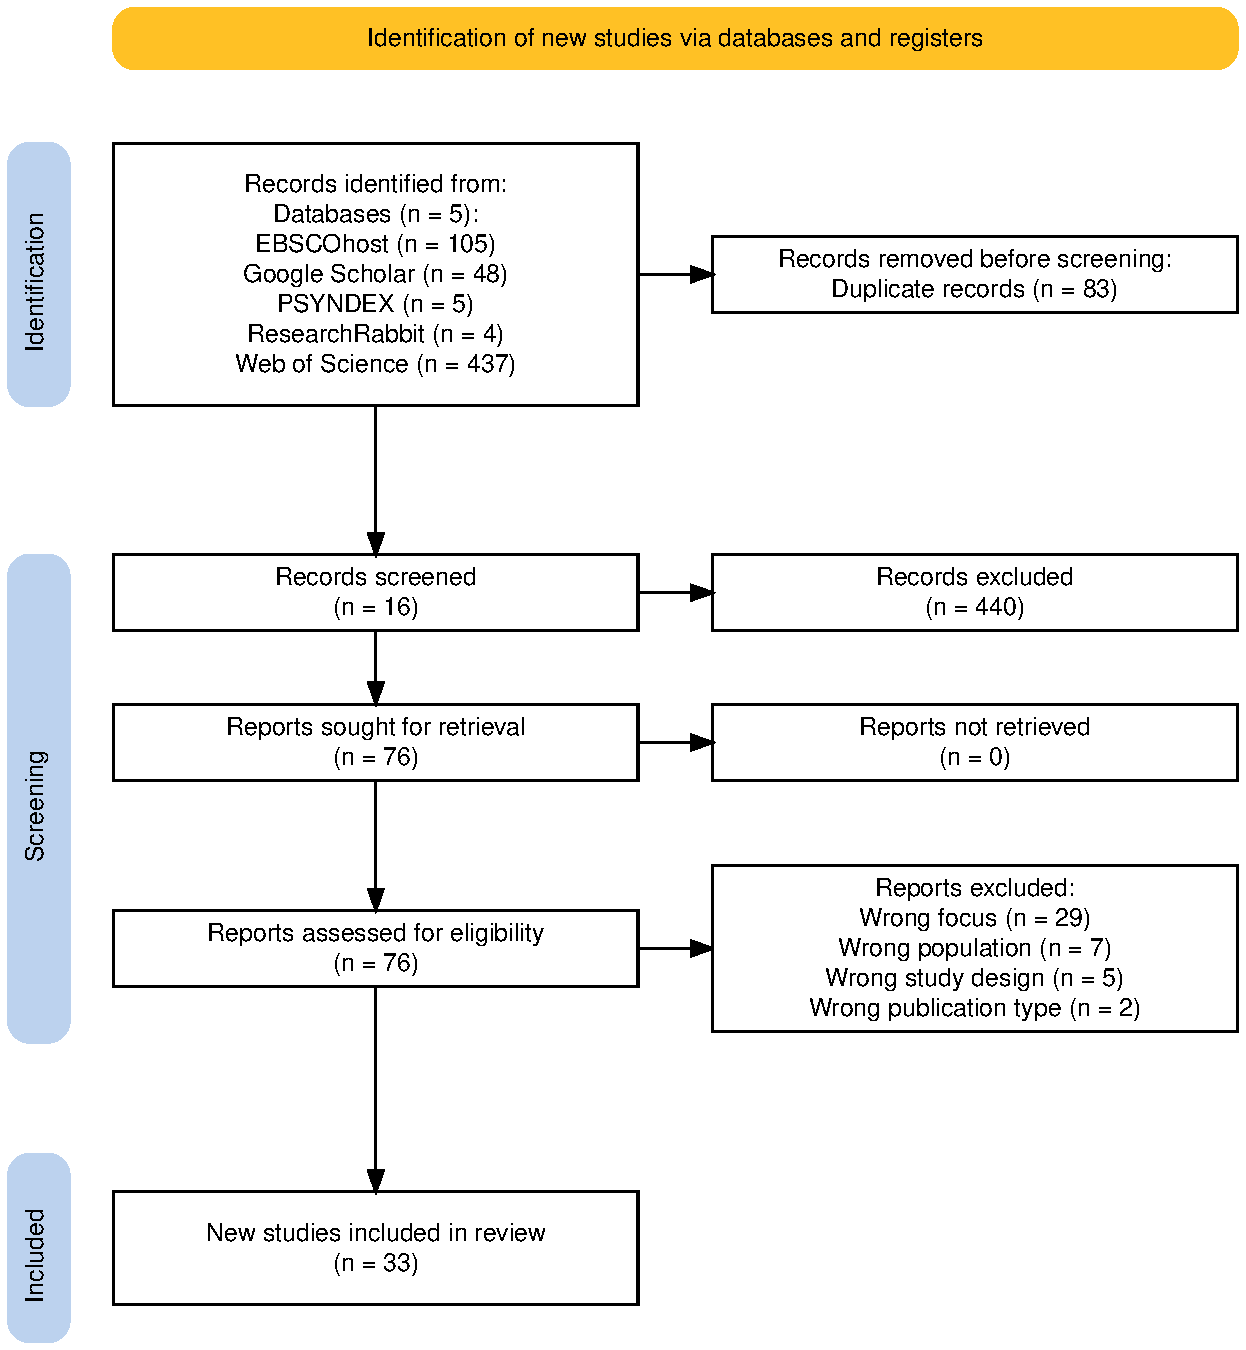
\includegraphics{files/prisma.pdf}
\caption{\label{fig:prisma}PRISMA flowchart of the screening process.}
\end{figure}

\subsection{RStudio and R packages}\label{rstudio-and-r-packages}

The following R packages were used to create this review: R (Version 4.4.1; R Core Team, 2024) and the R-packages \emph{citr} (Version 0.3.2; Aust, 2019), \emph{kableExtra} (Version 1.4.0; Zhu, 2024), \emph{papaja} (Version 0.1.2.9000; Aust \& Barth, 2023), \emph{RefManageR} (Version 1.4.0; McLean, 2017), \emph{rmarkdown} (Version 2.27; Xie et al., 2018, 2020), and \emph{tinylabels} (Version 0.2.4; Barth, 2023).

\section{Results}\label{results}

\subsection{Results Hypothesis 1: Stereotype threat induces variations in neutral activation across different brain areas and networks, potentially influencing academic performance.}\label{results-hypothesis-1-stereotype-threat-induces-variations-in-neutral-activation-across-different-brain-areas-and-networks-potentially-influencing-academic-performance.}

\subsubsection{Beilock et al. (2007)}\label{beilockstereotypethreatworking2007}

In their paper, Beilock et al. (2007) focussed on stereotypes effects on working memory, specifically, which parts of working memory are affected by stereotype threat and when these effects linger on and influence performance on unrelated tasks.
To investigate this, they focussed on maths stereotype threat, their population consisted of female college students in the United States.
Their paper describes five experiments, all of which used a cross-sectional design.
Experiment 1, 3 (both A and B), and Experiment 5, consisted of two groups each, with `stereotype threat' vs.~`no stereotype threat', `horizontal vs.~vertical modular arithmetic (MA) conditions', and `spatial two-back vs.~verbal two-back task', respectively, each with random allocation.
Experiment 2 and 4 consisted of one group each.
Since neither Experiment 2 nor 3B were relevant to the hypotheses for this review, they will not be discussed further.
Across all experiments, participants were female undergraduate students.

\paragraph{Modular Arithmetic (MA) task}\label{modular-arithmetic-ma-task}

The MA task was used to measure maths performance.
Participants were asked to judge the validity of equations, like \(60 = 19 mod(4)\), which would result in \(false\).
These equations were either displayed vertically or horizontally and consisted of varying difficulty, thus differed in working memory demand.
Using this type of task allowed the researchers to measure the effect stereotype threat had on working memory.

\paragraph{Two-back task}\label{two-back-task}

Participants were given a stimuli and had to decide whether or not the given stimuli matched the one presented two trials before.
The stimuli in use were a cluster of identical letters (e.g., \emph{cs}, \emph{ns}) and one of six different spatial locations in an ellipse.
The two-back task was split into a verbal (letters) or spatial (locations) version, participants were randomly assigned to one of these versions.

\paragraph{Experiment 1}\label{experiment-1}

\(N = 31\) women, of equal self-reported maths skill participated in this experiment, \(n_{\text{stereotype threat}} = 14\), \(n_{\text{no stereotype threat}} = 17\).
Firstly, participants were introduced to the MA task, and were then asked to solve 12 practice problems, these differed in demand but only consisted of horizontal problems.
Afterwards, 24 problems were performed by each participant over two blocks, with the first one serving as a baseline and the second as the posttest.
Stereotype threat manipulation was performed in between these blocks via text on a computer screen.
An adaptation of the stereotype threat manipulation used by Aronson et al. (1999) was used by displaying the text on a computer screen.
Maths accuracy and reaction time were measured as dependent variables, while Group (stereotype threat vs.~control), Problem working memory demand (low vs.~high), and Block (baseline vs.~posttest) functioned as independent variables.\\
Within the stereotype threat condition \(\text{Group } \times \text{ Block } \times \text{ Problem Demand }\), \emph{F}(1,29) = 11.18, \emph{p} \textless{} .010, \(\eta^{2}_{p}\) = 0.28, resulted in a significant interaction effect for accuracy.
Further, \(\text{Group } \times \text{ Block } \times \text{ Problem Demand }\), on reaction time, showed main effect of block, and problem demand; \emph{F}(1,29) = 8.33, \emph{p} \textless{} .010, \(\eta^{2}_{p}\) = 0.22, and \emph{F}(1,29) = 754.5, \emph{p} \textless{} .010, \(\eta^{2}_{p}\) = 0.96, respectively.
Thus, individuals were able to increase their speed over time and the more demanding a problem was, the longer it took to solve it.
A comparison of the accuracy between the baseline and posttest within the stereotype threat condition showed no difference in terms of accuracy for low-demand problems, while, for high-demand problems, a significant decrease in accuracy between the posttest (\emph{M} = 79.3\%, \emph{SE} = 4.6\%) and baseline (\emph{M} = 89.1\%, \emph{SE} = 3.8\%) was found; CI {[}81.00\% - 97.00\%{]}; \emph{d} = 0.61.\\
Beilock et al. (2007) conclude that only high- but not low-demand problems affect working memory under stereotype threat.

\paragraph{Experiment 3A}\label{experiment-3a}

Here, a sample of thirty-three (\(N = 33\)) women performed, both, vertical and horizontal MA tasks.
Similar to Experiment 1 they were introduced to the subject with a practice block, followed by a baseline block and a posttest block.
This time, all participants received the stereotype threat manipulation in between the last two blocks but were randomly assigned to either the vertical or horizontal problem condition.
Afterwards, they were given questionnaires to assess their thought during the stereotype threat manipulation, their perceived importance of task performance, and their state anxiety following stereotype threat.
The independent variables consisted of Block (baseline vs.~stereotype threat), Problem working memory demand (low vs.~high), and Problem orientation (horiztonal vs.~vertical), while the dependent variables were maths problem accuracy, reaction times, and self-reported thoughts/worries.
Neither the perceived importance of performing well (vertical: \emph{M} = 4.67, \emph{SE} = 0.35; horizontal: \emph{M} = 5.27, \emph{SE} = 0.37) nor state anxiety differed between the groups (vertical: \emph{M} = 33.22, \emph{SE} = 1.6; horizontal: \emph{M} = 37.00, \emph{SE} = 2.7), \emph{F}(1,31) = 1.53, \emph{p} = .220.
Thoughts/worries were split into four categories, most common were thoughts about the performance monitoring (34.9\%), followed by thoughts related about the processes involved in solving the problems (32.4\%), unrelated thoughts made up 18.3\% and, lastly, 14.5\% of the thoughts related to the stereotype threat manipulation.
Again, no significant difference between the groups was found (Categories 1, 3, and 4: \emph{F} \textless{} 1; Category 2: \emph{F}(1,31) = 2.17, \emph{p} = .150.)\\
For the MA problems, a three-way interaction between the independent variables was found, \emph{F}(1,31) = 4.12, \emph{p} = .050, \(\eta^{2}_{p}\) = 0.12.\\
Similar to Experiment 1, a significant \(\text{Block } \times \text{Problem Demand }\) interaction was found but only for horizontal problems, \emph{F}(1,14) = 7.70, \emph{p} \textless{} .020, \(\eta^{2}_{p}\) = 0.36.
Accuracy suffered significantly from the baseline (\emph{M} = 91.7\%, \emph{SE} = 3.6\%) to the stereotype threat (\emph{M} = 81.2\%, SE = 4.6\%) block; CI {[}84.00\% - 99.30\%{]}; \emph{d} = 0.64.
The three-way ANOVA for, RTs revealed that high-demand problems were slower, compared to low-demand problems; vertical: \emph{F}(1,17) = 306.32, \emph{p} \textless{} .010, \(\eta^{2}_{p}\) = 0.95; horizontal: \emph{F}(1,14) = 11.04, \emph{p} \textless{} .010, \(\eta^{2}_{p}\) = 0.44.
This effect was not significant for horizontal problems and revealed a main effect for vertical problems.\\
It is concluded that low-demand problems do not suffer under stereotype threat, however, the working memory is impaired for high-demand problems resulting in a decrease in accuracy (only for horizontal problems) and an increase in reaction time.

\paragraph{Experiment 4}\label{experiment-4}

All thirty (\(N = 30\)) women were tasked to solve horizontal and vertical MA under stereotype threat.
Procedure was similar to Experiment 3A, albeit, with a bigger practice block, and the repetition of some problems.
The independent variables consisted of Block (baseline vs.~stereotype threat), Problem Repetition (no repeat vs.~multiple repeat), and Problem Working Memory demand (low vs.~high), while the dependent variables did not differ from Experiment 1.\\
The significant \(\text{Block } \times \text{ Problem Repetition } \times \text{ Problem Working Memory demand }\) interaction, \emph{F}(1, 29) = 6.13, \emph{p} \textless{} .020, \(\eta^{2}_{p}\) = 0.17, was further analysed by differentiating between multi- and no=repeat problems.\\
For the multi-repeat problems no significant interaction was to be found (\emph{F} \textless{} 1), meanwhile a significant effect was found for the no-repeat problems, \emph{F}(1,29) = 11.11, \emph{p} \textless{} 0.01, \(\eta^{2}_{p}\) = 0.28.
While the accuracy, again, significantly decreased from the baseline (\emph{M} = 65.00\%, \emph{SE} = 3.9\%) to the stereotype threat block (\emph{M} = 65.00\%, \emph{SE} = 5.9\%; CI {[}52.80\% - 77.20\%{]}; \emph{d} = 0.70) in high-demand problems, within the no-repeat condition, no significant effect was found for the low-demand problems (baseline: \emph{M} = 95.00\%, \emph{SE} = 1.50\%, stereotype threat: \emph{M} = 94.80\%, \emph{SE} = 2.80\%).
For the RTs, problem demand, \emph{F}(1,26) = 144.14, \emph{p} \textless{} .010, \(\eta^{2}_{p}\) = 0.85, influenced the RTs more than problem repetition,\emph{F}(1,26) = 139.94, \emph{p} \textless{} .010, \(\eta^{2}_{p}\) = 0.84, both showing main effects.\\
Based on these results, the authors conclude that practised, horizontal problems do not rely on working memory heavily, evidenced by them not being affected by stereotype threat.
The opposite is true for no-repeat problems, which did suffer under stereotype threat, given that they were of high verbal working memory demand.

\paragraph{Experiment 5}\label{experiment-5}

The last experiment was preceded by a pilot test to establish whether the two-back tasks were of equal difficulty.
This pilot test was done with \(N = 27\) women, without any stereotype threat manipulation, the procedure is similar to the main experiment, thus will not be discussed further.\\
The main experiment consisted of thirty-three (\(N = 33\)) women.
Upon arrival participants completed a two-back practise task, after changing computers, they practised the MA task.
Afterwards, the stereotype threat manipulation was performed, followed by twenty high-demand horizontal problems.
In the next step, participants went back to the first computer to complete 100 trails of the same version of the two-back task that was practised before.\\
Condition (stereotype threat vs.~control; control being the pilot test) and Two-back task type (verbal vs.~spatial) functioned as independent variables, while the dependent variables were accuracy and reaction time, each for, both, the maths problem and the two-back task.\\
Comparing the MA results with the previous experiments results for the same type of task (horizontal, high-demand), showed that the stereotype threat significantly inhibited performance (\emph{M} = 82.20\%, \emph{SE} = 2.00\%), while the same cannot be said for the no-threat conditions (\emph{M} = 91.50\%, \emph{SE} = 1.50\%).\\
For the two-back task, RTs between spatial (\emph{M} = 895 ms, \emph{SE} = 49 ms) and verbal (\emph{M} = 1087 ms, \emph{SE} = 59 ms) task differed significantly, \emph{F}(1,31) = 6.133, \emph{p} \textless{} .020, \(\eta^{2}_{p}\) = 0.17 while the difference in accuracy did not reach significance (verbal: \emph{M} = 87.30\%, \emph{SE} = 1.70\%; spatial: \emph{M} = 89.00\%, \emph{SE} = 1.50\%, \emph{F} \textless{} 1).
Comparing the performance of the stereotype threat condition with the control (pilot test), showed an interaction between \(\text{Task } \times \text{ Experiment }\) for RT, \emph{F}(1,56) = 4.38, \emph{p} \textless{} .050, \(\eta^{2}_{p}\) = 0.07.
Without stereotype threat, no significant differences in performance between thee verbal and spatial two-back tasks were found, however, under stereotype threat the verbal task was significantly slower than the spatial task.\\
Contrary to the previous Experiments, Experiment 5 additionally aimed to investigate whether stereotype threat has a spill over effect on unrelated tasks.
Since these results are not relevant to the hypotheses of this review, they will not be discussed in detail.
Using multiple regression analyses the authors found that the stereotype threat did indeed spill over to the two-back task, however, only for the verbal task.\\
According to the authors, the results of the different Experiments in this paper, show stereotype threats effect on working memory, they mention that ``especially the phonological aspects'' are affected.
Stereotype threat's effect onto task-related worries as well as thoughts serve as further indications for this conclusion.
Further, it is concluded that stereotype threat likely affects multiple aspects of working memory.
A combination of phonological loop and central executive functioning is suggested to be affected by stereotype threat.\\
H1 is partially confirmed by this paper, central executive functioning is assumed to involve the prefrontal cortex, however, this is not the only area affected.
The phonological loop is associated with BA4, BA49, and (approximately) BA44 and BA 45.

\subsubsection{Dunst et al. (2013)}\label{dunstsexdifferencesneural2013}

In a \(2 \text{ (sex: male vs. female) } \times 2 \text{ (stereotype exposure: stereotype threat vs. no stereotype threat) }\) cross-sectional between-subjects design, a mixed-sex sample of secondary school students in Austria, was used to investigate the effects of stereotype threat on neural efficiency as well as sex differences in visuo-spatial task performance.
The dependent variables consisted of task performance (accuracy and reaction time), brain activation (task-related-power changes), and neural efficiency (correlation between figural intelligence and brain activation); sex, stereotype exposure, and figural intelligence functioned as independent variables.
Task-related-power (TRP) changes were measured using an EEG, specifically the upper alpha band (10-12 Hz) were examined.\\
The final sample consisted of 58 participants (\(N = 58\); 26 girls, 32 boys).
Participants were randomly assigned to either the stereotype threat or control conditions, additionally, they were IQ-matched between experimental groups.\\
Firstly, participants were set up with the EEG, 33 electrodes were placed, following the international 10-20 system.
Afterwards, the stereotype threat manipulation was performed using a message claiming boys to be better on the subsequent task, in the no-threat condition the message was neutral, stating that sex differences did not exist.
Previous studies successfully used a similar manipulation in the past.\\
None of the behavioural analyses were significant, since they do not relate to this reviews hypotheses, they will not be discussed further.
The TRP changes were analysed, a main effect for Stereotype Exposure (\emph{F}(1,54) = 3.93, \emph{p} = .050, \(\text{partial }\eta^{2}\) = 0.07) was found using a four-way ANOVA, with the between-subjects factors of Stereotype Exposure, and Sex and the within-subjects factors of Hemisphere and Area.
A higher cortical activation (\emph{M} = 0.07, \emph{SD} = 0.03) was found in the stereotype threat condition compared to the control condition (\emph{M} = -0.03, \emph{SD} = 0.03).

\section{Discussion}\label{discussion}

\newpage

\section{References}\label{references}

\phantomsection\label{refs}
\begin{CSLReferences}{1}{0}
\bibitem[\citeproctext]{ref-anthropicClaudeAiSonnet2024}
Anthropic. (2024). \emph{Claude {Ai} 3.5 {Sonnet}}. https://claude.ai/.

\bibitem[\citeproctext]{ref-aronsonWhenWhiteMen1999}
Aronson, J., Lustina, M. J., Good, C., Keough, K., Steele, C. M., \& Brown, J. (1999). When white men can't do math: {Necessary} and sufficient factors in stereotype threat. \emph{Journal of Experimental Social Psychology}, \emph{35}(1), 29--46. \url{https://doi.org/10.1006/jesp.1998.1371}

\bibitem[\citeproctext]{ref-R-citr}
Aust, F. (2019). \emph{Citr: 'RStudio' add-in to insert markdown citations}. \url{https://github.com/crsh/citr}

\bibitem[\citeproctext]{ref-R-papaja}
Aust, F., \& Barth, M. (2023). \emph{{papaja}: {Prepare} reproducible {APA} journal articles with {R Markdown}}. \url{https://github.com/crsh/papaja}

\bibitem[\citeproctext]{ref-R-tinylabels}
Barth, M. (2023). \emph{{tinylabels}: Lightweight variable labels}. \url{https://cran.r-project.org/package=tinylabels}

\bibitem[\citeproctext]{ref-beilockStereotypeThreatWorking2007}
Beilock, S. L., Rydell, R. J., \& McConnell, A. R. (2007). Stereotype threat and working memory: {Mechanisms}, alleviation, and spillover. \emph{Journal of Experimental Psychology: General}, \emph{136}(2), 256--276. \url{https://doi.org/10.1037/0096-3445.136.2.256}

\bibitem[\citeproctext]{ref-criticalappraisalskillsprogrammeCASPSystematicReview2018}
Critical Appraisal Skills Programme. (2018). {CASP Systematic Review Checklist} {[}Organization{]}. In \emph{CASP - Critical Appraisal Skills Programme}. https://casp-uk.net/casp-tools-checklists/.

\bibitem[\citeproctext]{ref-dunstSexDifferencesNeural2013}
Dunst, B., Benedek, M., Bergner, S., Athenstaedt, U., \& Neubauer, A. C. (2013). Sex differences in neural efficiency: {Are} they due to the stereotype threat effect? \emph{Personality and Individual Differences}, \emph{55}(7), 744--749. \url{https://doi.org/10.1016/j.paid.2013.06.007}

\bibitem[\citeproctext]{ref-eppi-centreReviewGuidelinesExtracting2003}
EPPI-Centre. (2003). \emph{Review guidelines for extracting data and quality assessing primary studies in educational research} (Guidelines Version 0.9.7). Social Science Research Unit.

\bibitem[\citeproctext]{ref-githubGitHubCopilot2024}
GitHub, \& OpenAi. (2024). \emph{{GitHub Copilot}}. copilot.github.com.

\bibitem[\citeproctext]{ref-lakensImprovingYourStatistical2022}
Lakens, D. (2022). \emph{Improving {Your Statistical Inferences}}. Zenodo. \url{https://doi.org/10.5281/ZENODO.6409077}

\bibitem[\citeproctext]{ref-R-RefManageR}
McLean, M. W. (2017). RefManageR: Import and manage BibTeX and BibLaTeX references in r. \emph{The Journal of Open Source Software}. \url{https://doi.org/10.21105/joss.00338}

\bibitem[\citeproctext]{ref-ouzzaniRayyanWebMobile2016}
Ouzzani, M., Hammady, H., Fedorowicz, Z., \& Elmagarmid, A. (2016). Rayyan---a web and mobile app for systematic reviews. \emph{Systematic Reviews}, \emph{5}(1), 210. \url{https://doi.org/10.1186/s13643-016-0384-4}

\bibitem[\citeproctext]{ref-positteamRStudioIntegratedDevelopment2024}
Posit team. (2024). \emph{{RStudio}: {Integrated} development environment for {R}} {[}Manual{]}. Posit Software, PBC.

\bibitem[\citeproctext]{ref-R-base}
R Core Team. (2024). \emph{R: A language and environment for statistical computing}. R Foundation for Statistical Computing. \url{https://www.R-project.org/}

\bibitem[\citeproctext]{ref-universityofglasgowCriticalAppraisalChecklistn.d.nodate}
University of Glasgow. (n.d.). \emph{Critical appraisal checklist for a systematic review} {[}Checklist{]}. Department of General Practice, University of Glasgow.

\bibitem[\citeproctext]{ref-wellsNewcastleottawaScaleNOS2014}
Wells, G., Shea, B., O'Connell, D., Robertson, J., Welch, V., Losos, M., \& Tugwell, P. (2014). The newcastle-ottawa scale ({NOS}) for assessing the quality of nonrandomised studies in meta-analyses. \emph{Ottawa Health Research Institute Web Site}, \emph{7}.

\bibitem[\citeproctext]{ref-R-rmarkdown_a}
Xie, Y., Allaire, J. J., \& Grolemund, G. (2018). \emph{R markdown: The definitive guide}. Chapman; Hall/CRC. \url{https://bookdown.org/yihui/rmarkdown}

\bibitem[\citeproctext]{ref-R-rmarkdown_b}
Xie, Y., Dervieux, C., \& Riederer, E. (2020). \emph{R markdown cookbook}. Chapman; Hall/CRC. \url{https://bookdown.org/yihui/rmarkdown-cookbook}

\bibitem[\citeproctext]{ref-R-kableExtra}
Zhu, H. (2024). \emph{kableExtra: Construct complex table with 'kable' and pipe syntax}. \url{https://CRAN.R-project.org/package=kableExtra}

\end{CSLReferences}


\clearpage
\renewcommand{\listfigurename}{Figure captions}

\clearpage
\renewcommand{\listtablename}{Table captions}


\end{document}
